\documentclass[tikz,border=10pt]{standalone}
\usepackage{amsmath}
\usetikzlibrary{arrows.meta}
\begin{document}
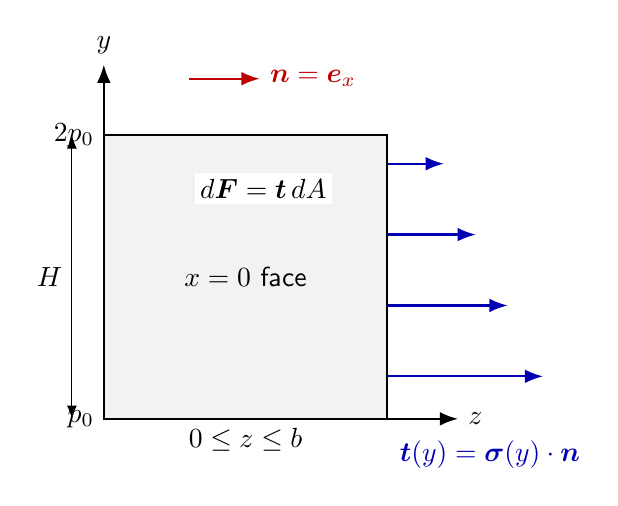
\begin{tikzpicture}[>=Latex,font=\sffamily,scale=0.9]
\filldraw[fill=gray!10,draw=black,thick] (0,0) rectangle (4,4);
\draw[->,thick] (0,0) -- (0,5) node[above] {$y$};
\draw[->,thick] (0,0) -- (5,0) node[right] {$z$};
\draw[->,thick,blue!70!black] (4,0.6) -- (6.2,0.6);
\draw[->,thick,blue!70!black] (4,1.6) -- (5.7,1.6);
\draw[->,thick,blue!70!black] (4,2.6) -- (5.25,2.6);
\draw[->,thick,blue!70!black] (4,3.6) -- (4.8,3.6);
\node[blue!70!black,align=center] at (5.45,-0.5) {$\boldsymbol t(y)=\boldsymbol\sigma(y)\cdot\boldsymbol n$};
\node at (2,2) {$x=0$ face};
\node[left] at (0,0) {$p_0$};
\node[left] at (0,4) {$2p_0$};
\node[below] at (2,0) {$0\le z\le b$};
\node[fill=white,inner sep=2pt] at (2.25,3.25) {$d\boldsymbol F=\boldsymbol t\,dA$};
\draw[<->] (-0.45,0) -- (-0.45,4) node[midway,left] {$H$};
\draw[->,thick,red!75!black] (1.2,4.8) -- (2.2,4.8) node[right] {$\boldsymbol n=\boldsymbol e_x$};
\end{tikzpicture}
\end{document}
